\documentclass[10pt,a4paper]{article}
\usepackage[T1]{fontenc}
\usepackage[utf8]{inputenc}
\usepackage[french]{babel}
\usepackage{lmodern}
\usepackage[margin=1.8cm,top=2.1cm,bottom=1.8cm,headsep=0.4cm,headheight=13pt]{geometry}
\usepackage{graphicx}
\usepackage{booktabs}
\usepackage{caption}
\usepackage{microtype}
\usepackage{xcolor}
\usepackage{enumitem}
\usepackage{amssymb}
\usepackage[hidelinks]{hyperref}
\usepackage{fancyhdr}

\pagestyle{fancy}
\fancyhf{}
\fancyhead[L]{\small Reproduction de Cosme, Thomas \& Gaucherel (2023)}
\fancyhead[R]{\small Benbakreti \& Ben Romdhane}
\fancyfoot[C]{\small\thepage}

\captionsetup{font=small,labelfont=bf,skip=4pt}
\addto\captionsfrench{\renewcommand{\tablename}{Tableau}}
\setlist{nosep,leftmargin=*}
\setlength{\parskip}{0.35em}
\setlength{\parindent}{0pt}
\newcommand{\titre}[1]{\par\vspace{0.5em}{\large\bfseries #1}\par\vspace{0.15em}}
\newcommand{\ecco}{\texttt{ecco}}
\newcommand{\vide}{$\varnothing$}

\begin{document}

% Page de garde : hors des 3 pages du rapport (la numérotation repart à 1 après elle)
\begin{titlepage}
\centering
\vspace*{0.8cm}
{\Large Université Paris-Saclay\par}
\vspace{0.4em}
{\large Master 2 Informatique\par}
\vspace{0.3em}
{\normalsize Projet de reproduction d'article\par}
\vfill
{\huge\bfseries Reproduction des figures 5 et 7\\[0.3em] de Cosme, Thomas \& Gaucherel (2023)\par}
\vspace{1.2em}
{\Large Modèle qualitatif APT : exécution synchrone\\[0.2em] et asynchrone avec \ecco\par}
\vspace{2.2em}
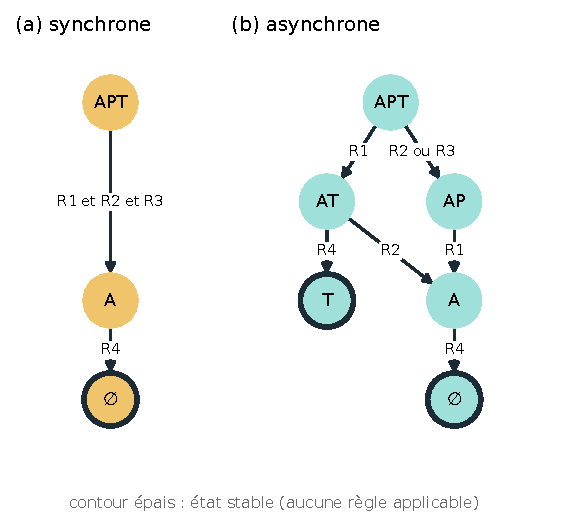
\includegraphics[width=0.6\textwidth]{../figures/figure7_sync_async.pdf}\\[0.3em]
{\small Graphes d'états depuis \{APT\} : (a) synchrone, (b) asynchrone\par}
\vfill
{\large\bfseries Mohammed El Amine BENBAKRETI\\[0.5em] Mohamed Aziz BEN ROMDHANE\par}
\vspace{2.5em}
\begin{minipage}{0.82\textwidth}
\centering\small\NoAutoSpacing
Article étudié : M.~Cosme, C.~Thomas, C.~Gaucherel. \emph{On the History of Ecosystem Dynamical Modeling: The Rise and Promises of Qualitative Models.} Entropy 25(11):1526, 2023. doi:10.3390/e25111526
\end{minipage}
\par\vspace{1.8em}
{\large\today\par}
\vspace*{0.6cm}
\end{titlepage}

\titre{Contexte}
Pour modéliser un écosystème, on écrit le plus souvent des équations différentielles dont les paramètres (taux de croissance, de prédation\dots) doivent être mesurés. En écologie, ces mesures sont rares, coûteuses et varient dans le temps. Les modèles \emph{qualitatifs} contournent ce problème : chaque espèce est seulement présente ($+$) ou absente ($-$), et des règles « si\dots{} alors\dots{} » décrivent les événements possibles, par exemple « si l'amibe A est présente, la paramécie P peut disparaître ». L'outil \ecco{} (F.~Pommereau, IBISC) lit ces règles et calcule le \emph{graphe de transitions d'états} (STG) : tous les états accessibles depuis un état initial, reliés par les événements qui y mènent. Ce travail reproduit les deux expériences de l'article, menées sur un modèle de trois protistes (APT) : le STG depuis l'état \{APT\} (Fig.~5) et l'effet du mode d'exécution des règles, synchrone ou asynchrone (Fig.~7).

\titre{1. De quoi parle l'article ?}
L'article~[1] est d'abord une \textbf{revue historique} doublée d'un \textbf{plaidoyer méthodologique}. Il retrace la modélisation dynamique des écosystèmes depuis les années 1950 : modèles à compartiments en équations différentielles, approches thermodynamiques, puis une lignée qualitative plus discrète. Celle-ci part des « réseaux de réactions » de Camerano (1880), passe par la \emph{loop analysis} de Levins et le raisonnement qualitatif (QSIM, Garp3), et aboutit aux modèles état-transition de la gestion des parcours. Chaque formalisme y est présenté comme un assemblage de propriétés : quantitatif ou qualitatif, mise à jour synchrone ou non, déterministe, probabiliste ou possibiliste. Ces assemblages sont jugés selon quatre objectifs : (1)~saisir la dynamique qualitative, (2)~faire le moins d'hypothèses possible sur les paramètres, (3)~expliquer, (4)~prédire.

Les auteurs en déduisent le cadre \textbf{EDEN} (\emph{Ecological Discrete-Event Networks}), implémenté dans \ecco. EDEN combine des variables qualitatives (un seuil de fonctionnalité sépare présent et absent), des \textbf{événements discrets} au lieu d'une horloge globale, une mise à jour \textbf{asynchrone} (une règle à la fois) et une vision \textbf{possibiliste} (toutes les trajectoires sont calculées, sans probabilités). Le STG obtenu s'analyse par sa topologie (composantes fortement connexes, états stables, bassins) ou par \emph{model-checking}. Le seul matériau expérimental est le modèle APT. Il comprend trois protistes, \emph{Amoeba proteus}~(A), \emph{Paramecium caudatum}~(P) et \emph{Tetrahymena pyriformis}~(T), et quatre règles : R1~: $A{+}\to P{-}$, R2~: $A{+}\to T{-}$, R3~: $P{+}\to T{-}$, R4~: $P{-}\to A{-}$. Il illustre la thèse centrale : un modèle qualitatif \emph{synchrone} suppose que tous les processus vont à la même vitesse, et peut ainsi faire rejeter un modèle pourtant correct.

\titre{2. Quelles réponses, avec quelle confiance ?}
\textbf{Méthode.} L'article ne fournit ni fichier de modèle ni code. Nous avons donc écrit le modèle au format \texttt{.rr} d'\ecco{} à partir de la Fig.~5b (\texttt{APT.rr} : trois variables présentes au départ et les règles R1--R4), puis travaillé dans \ecco{} Jupyter avec deux notebooks. \texttt{ecco.load} lit le fichier. \texttt{model()} calcule l'espace des états accessibles depuis \{APT\}, d'abord regroupé en une seule composante. \texttt{explicit()} sépare cette composante en un nœud par état, et \texttt{draw()} affiche le graphe. Les figures~1 et~2 reprennent ces graphes avec le nom des états à la place des numéros d'\ecco. \ecco{} exécute les règles une à une et n'a pas de mode synchrone. Pour la Fig.~7a, nous avons donc regroupé à la main les règles tirées ensemble en deux règles, dans \texttt{APT\_synchrone.rr} : S1~: $A{+},P{+},T{+}\to P{-},T{-}$ (R1, R2 et R3 depuis \{APT\}) et S2~: $A{+},P{-},T{-}\to A{-}$ (R4 depuis \{A\}).

\begin{figure}[!htb]
\centering
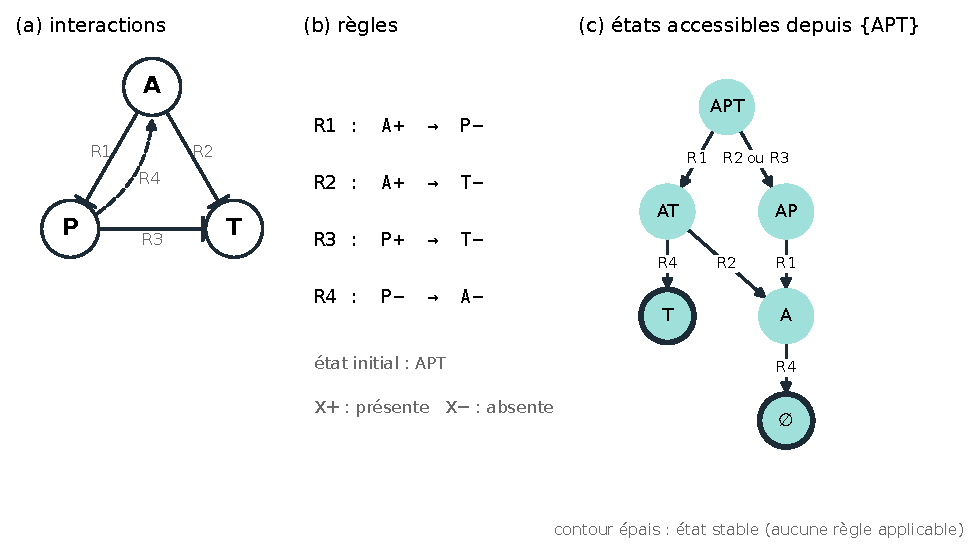
\includegraphics[width=0.86\textwidth]{../figures/figure5_APT.pdf}
\caption{Reproduction de la figure 5. (a)~Interactions déduites des règles ($\dashv$ : X fait disparaître Y) ; la dépendance en pointillés (R4 : A dépend de P) n'est pas dessinée dans l'article. (b)~Règles. (c)~Graphe d'états asynchrone depuis \{APT\}, le même que celui affiché par \ecco{} : 6 états, 6 transitions ; les états stables \{T\} et \vide{} ont un contour épais.}
\end{figure}

\textbf{Résultats.} Les graphes calculés par \ecco{} correspondent aux figures de l'article (tableau~1). En \textbf{asynchrone} (Fig.~1c), on obtient les 6 états et les 6 transitions de la Fig.~5c, étiquettes comprises (APT$\to$AP par « R2, R3 »). Il y a deux états stables, \{T\} et \vide, et trois trajectoires : APT$\to$AT$\to$T, APT$\to$AT$\to$A$\to$\vide{} et APT$\to$AP$\to$A$\to$\vide. En \textbf{synchrone} (Fig.~2a), la seule trajectoire est APT$\to$A$\to$\vide, comme dans la Fig.~7a.

Le graphe rend aussi le mécanisme explicite. Pour que T survive, R1 (A mange P) puis R4 (A disparaît faute de P) doivent se produire avant R2 (A mange T) ; depuis AT, R3 ne s'applique plus. Depuis AP, seule l'issue \vide{} reste possible ; depuis AT, les deux issues le restent. L'extinction de P est donc nécessaire mais pas suffisante pour aboutir à \{T\}, comme l'affirme l'article. Le mode synchrone interdit cet ordre, puisqu'il fait manger P et T par A au même instant.

\begin{figure}[!htb]
\begin{minipage}[c]{0.44\textwidth}
\centering
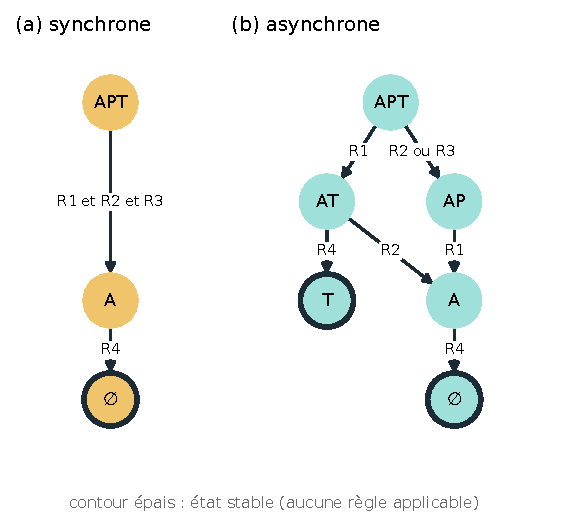
\includegraphics[width=\linewidth]{../figures/figure7_sync_async.pdf}
\caption{Reproduction de la figure 7 : même modèle, même état initial, exécution (a)~synchrone et (b)~asynchrone.}
\end{minipage}\hfill
\begin{minipage}[c]{0.53\textwidth}
\centering
\captionsetup{justification=centering}
\captionof{table}{Résultats lus sur les graphes \ecco.}
\small
\begin{tabular}{@{}lcccc@{}}
\toprule
mode & états & trans. & stables & traj. \\
\midrule
synchrone & 3 & 2 & \vide & 1 \\
asynchrone & 6 & 6 & \{T\}, \vide & 3 \\
\bottomrule
\end{tabular}

\vspace{1.2em}
\begin{tabular}{@{}p{0.74\linewidth}l@{}}
\toprule
Affirmation de l'article & constaté \\
\midrule
STG de la Fig.~5c (arcs et règles) & \checkmark \\
2 états stables, 4 transitoires & \checkmark \\
3 trajectoires alternatives & \checkmark \\
P éteinte : nécessaire, non suffisante pour \{T\} & \checkmark \\
Synchrone : APT$\to$A$\to$\vide{} (Fig.~7a) & \checkmark \\
\{T\} observé expérimentalement & non vérif. \\
\bottomrule
\end{tabular}
\end{minipage}
\end{figure}

\textbf{Confiance et limites.} Notre confiance est \textbf{élevée pour le graphe asynchrone}. Le STG découle de façon déterministe des quatre règles : on peut le vérifier à la main sur 8 états, et le graphe calculé par \ecco{} coïncide arc par arc avec la Fig.~5c. Elle est \textbf{bien plus faible pour la conclusion écologique}, que l'article appuie sur ce seul exemple.
\begin{enumerate}
\item \emph{Synchrone codé à la main.} Nos règles S1 et S2 ne valent que pour la trajectoire partant de \{APT\}, et nous les avons écrites en connaissant la Fig.~7a : c'est une illustration, pas un mode synchrone générique. Depuis AT par exemple, un vrai pas synchrone (R2 et R4 ensemble) mènerait à \vide, alors qu'aucune de nos règles ne s'y applique.
\item \emph{Expériences minimalistes.} L'article est d'abord une revue. Son unique exemple compte 3 variables et 4 règles, sans comparaison avec un autre formalisme sur les mêmes données ni étude de sensibilité aux règles.
\item \emph{Une seule étude expérimentale.} \{T\} est observé dans les microcosmes de Weatherby \emph{et al.}~[2]. L'affirmation la plus forte (« toutes les transitions observées sont prédites ») renvoie à une prépublication des mêmes auteurs~[3], citée comme \emph{submitted}. L'article ne donne aucun chiffre : ni nombre de réplicats, ni fréquence des issues \{T\} et \vide. De plus, le modèle est « dérivé » de ces mêmes expériences, si bien que la validation n'est pas indépendante.
\item \emph{Comparaison binaire.} Opposer le synchrone strict à l'asynchrone montre que le mode de mise à jour change les conclusions, pas que l'asynchrone est le bon choix en général. Il existe d'autres schémas : mode semi-synchrone (mentionné mais \emph{not shown}), asynchrone généralisé, priorités via les contraintes d'\ecco~[4,6].
\item \emph{Possible n'est pas probable.} Le possibilisme ne distingue pas une issue fréquente d'une issue rare. Sur un grand modèle, l'asynchrone peut aussi créer des trajectoires irréalistes et faire exploser le nombre d'états, ce que les auteurs reconnaissent.
\item \emph{Reproductibilité.} La légende de la Fig.~7 renvoie par erreur à la Fig.~6 au lieu de la Fig.~5. Le dépôt GitHub cité pour \ecco{} est aujourd'hui archivé ; le code a migré sur Codeberg~[5].
\end{enumerate}

\titre{3. Quelles perspectives ?}
\begin{itemize}
\item \textbf{Élargir la validation} : appliquer la démarche aux autres combinaisons d'espèces du même pool expérimental~[2,7], puis compter systématiquement les états prédits mais non observés et les états observés mais non prédits.
\item \textbf{Mesurer ce que le possibilisme laisse de côté} : attacher des taux aux transitions du même STG (chaîne de Markov), estimer la probabilité d'aboutir à \{T\} et la confronter aux fréquences observées.
\item \textbf{Comparer les schémas de mise à jour} (synchrone, semi-synchrone, asynchrone généralisé), et tester la robustesse des conclusions en retirant ou modifiant une règle à la fois.
\item \textbf{Exploiter les analyses d'\ecco} : \emph{model-checking} CTL (« toute trajectoire vers \{T\} passe-t-elle par AT ? »), regroupement en composantes pour les grands modèles.
\item \textbf{Apprendre les règles à partir des données} au lieu de les écrire à la main, comme le proposent des travaux récents sur les réseaux booléens écologiques~[8]. Côté outil, un mode synchrone natif dans \ecco{} éviterait de coder le synchrone à la main comme nous l'avons fait.
\end{itemize}

\titre{Références}
{\footnotesize\NoAutoSpacing
\begin{enumerate}[label={[\arabic*]}]
\item M. Cosme, C. Thomas, C. Gaucherel. On the history of ecosystem dynamical modeling: the rise and promises of qualitative models. \emph{Entropy} 25(11):1526, 2023. doi:10.3390/e25111526
\item A.J. Weatherby, P.H. Warren, R. Law. Coexistence and collapse: an experimental investigation of the persistent communities of a protist species pool. \emph{J. Anim. Ecol.} 67:554--566, 1998.
\item M. de Goër de Herve, C. Thomas, M. Cosme, P.H. Warren, C. Gaucherel. Is a community state reachable, and why? Prépublication Authorea, 2022. doi:10.22541/au.164301558.85072720/v1
\item C. Gaucherel, F. Pommereau. Using discrete systems to exhaustively characterize the dynamics of an integrated ecosystem. \emph{Methods Ecol. Evol.} 10:1615--1627, 2019.
\item F. Pommereau. \ecco{} : \url{https://codeberg.org/fpom/ecco} (ex-\url{https://github.com/fpom/ecco}).
\item A. Garg, A. Di Cara, I. Xenarios, L. Mendoza, G. De Micheli. Synchronous versus asynchronous modeling of gene regulatory networks. \emph{Bioinformatics} 24:1917--1925, 2008.
\item P.H. Warren, R. Law, A.J. Weatherby. Mapping the assembly of protist communities in microcosms. \emph{Ecology} 84:1001--1011, 2003.
\item L. Paulevé, C. Gaucherel. Inference of ecological networks and possibilistic dynamics based on Boolean networks from observations and prior knowledge. \emph{Methods Ecol. Evol.}, doi:10.1111/2041-210X.70090 (prépublication bioRxiv 2024).
\end{enumerate}}

\end{document}
